% ============================================================
% 初升高衔接讲义 7 —— 集合概念预习
% 编译命令：xelatex -interaction=nonstopmode 衔接7_集合概念预习.tex
% ============================================================
\documentclass[12pt, a4paper]{ctexart}
\usepackage[margin=2.2cm]{geometry}
\usepackage{amsmath, amssymb}
\usepackage{enumitem}
\usepackage{tcolorbox}
\usepackage{booktabs}
\usepackage{array}
\usepackage{fancyhdr}
\usepackage{xcolor}
\usepackage{tikz}
\usepackage{hyperref}
\usepackage{graphicx}
\usepackage{multirow}
\usepackage{pgfplots}
\pgfplotsset{compat=1.18}

% 颜色定义
\definecolor{mainblue}{RGB}{41, 98, 168}
\definecolor{lightblue}{RGB}{230, 240, 255}
\definecolor{tipgreen}{RGB}{34, 139, 87}
\definecolor{lightgreen}{RGB}{235, 250, 240}
\definecolor{warnred}{RGB}{200, 50, 50}
\definecolor{lightred}{RGB}{255, 240, 240}
\definecolor{examorange}{RGB}{210, 120, 20}
\definecolor{lightorange}{RGB}{255, 248, 235}
\definecolor{apppurple}{RGB}{120, 60, 170}
\definecolor{lightpurple}{RGB}{245, 238, 255}

% 页眉页脚
\pagestyle{fancy}
\fancyhf{}
\fancyhead[L]{\small\textcolor{mainblue}{\textbf{初升高衔接·第7讲\quad 集合概念预习}}}
\fancyhead[R]{\small\textcolor{mainblue}{衔接讲义}}
\fancyfoot[C]{\small —\ \thepage\ —}
\renewcommand{\headrulewidth}{0.6pt}
\renewcommand{\headrule}{\hbox to\headwidth{\color{mainblue}\leaders\hrule height \headrulewidth\hfill}}
\renewcommand{\footrulewidth}{0pt}

% tcolorbox 样式
\newtcolorbox{knowledgebox}[1][]{%
  colback=lightblue, colframe=mainblue,
  fonttitle=\bfseries\large, title=#1,
  arc=3mm, boxrule=0.8pt,
  left=8pt, right=8pt, top=6pt, bottom=6pt
}

\newtcolorbox{tipbox}[1][]{%
  colback=lightgreen, colframe=tipgreen,
  fonttitle=\bfseries, title=#1,
  arc=2mm, boxrule=0.6pt,
  left=6pt, right=6pt, top=4pt, bottom=4pt
}

\newtcolorbox{warnbox}[1][]{%
  colback=lightred, colframe=warnred,
  fonttitle=\bfseries, title=#1,
  arc=2mm, boxrule=0.6pt,
  left=6pt, right=6pt, top=4pt, bottom=4pt
}

\newtcolorbox{examplebox}[1][]{%
  colback=lightorange, colframe=examorange,
  fonttitle=\bfseries, title=#1,
  arc=3mm, boxrule=0.8pt,
  left=8pt, right=8pt, top=6pt, bottom=6pt
}

\newtcolorbox{appbox}[1][]{%
  colback=lightpurple, colframe=apppurple,
  fonttitle=\bfseries, title=#1,
  arc=3mm, boxrule=0.8pt,
  left=8pt, right=8pt, top=6pt, bottom=6pt
}

\setCJKmainfont{Hiragino Sans GB}
\setCJKsansfont{Heiti SC}

\begin{document}

% ============ 标题页 ============
\begin{center}
{\Huge\bfseries\textcolor{mainblue}{第7讲\quad 集合概念预习}}\\[12pt]
{\Large\textcolor{gray}{初升高衔接讲义}}\\[8pt]
\rule{0.6\textwidth}{1pt}\\[8pt]
{\normalsize 适用：准高一新生\quad |\quad 课时：2课时}
\end{center}
\vspace{10pt}

% ================================================================
%  第一部分：知识点讲解
% ================================================================
\section*{\textcolor{mainblue}{一、知识点讲解}}

% ---------- 1.1 集合的概念 ----------
\subsection*{1.1\quad 集合的概念}

\begin{knowledgebox}[什么是集合]
\textbf{集合}（Set）是指满足某些\textbf{特定条件}的对象的\textbf{总体}。集合中的每个对象叫做这个集合的\textbf{元素}。

例如：
\begin{itemize}[leftmargin=2em]
  \item "我们班所有同学"构成一个集合，每个同学是元素；
  \item "大于0且小于10的偶数"构成集合 $\{2,4,6,8\}$。
\end{itemize}
\end{knowledgebox}

集合有三大特性：

\begin{enumerate}[leftmargin=2.5em]
  \item \textbf{确定性}：对于任何一个对象，能明确判断它\textbf{属于}还是\textbf{不属于}这个集合。
        \quad\textit{（例如："高个子同学"不能构成集合，因为"高个子"没有明确标准。）}
  \item \textbf{互异性}：集合中的元素\textbf{互不相同}。重复出现的元素只算一个。
        \quad\textit{（例如：$\{1,1,2\}$ 应写成 $\{1,2\}$。）}
  \item \textbf{无序性}：集合中的元素\textbf{没有先后顺序}。
        \quad\textit{（例如：$\{1,2,3\}$ 和 $\{3,1,2\}$ 表示同一个集合。）}
\end{enumerate}

\begin{warnbox}[易错提醒]
\begin{itemize}[leftmargin=2em]
  \item "约等于3的数"不能构成集合——不满足确定性。
  \item 集合 $\{x^2,\, x\}$ 中两个元素必须不同，即 $x^2 \neq x$，解得 $x\neq 0$ 且 $x\neq 1$。如果题目隐含此集合合法，说明 $x$ 的取值已经排除了这些值。
\end{itemize}
\end{warnbox}

% ---------- 1.2 集合的表示方法 ----------
\subsection*{1.2\quad 集合的表示方法}

\begin{knowledgebox}[两种常用表示方法]

\textbf{方法一：列举法}

把集合中的元素\textbf{一一写出来}，放在大括号 $\{\ \}$ 内。

\[
A = \{1,\, 2,\, 3,\, 4,\, 5\}, \qquad
B = \{a,\, b,\, c\}
\]

如果元素有明显规律且数量多，可以用省略号：
\[
C = \{1,\, 2,\, 3,\, \cdots,\, 100\}
\]

\vspace{6pt}
\textbf{方法二：描述法}

用文字或数学符号\textbf{描述元素的共同特征}，格式为：
\[
\{\, x \mid P(x) \,\}
\]
其中 $x$ 是代表元素，$P(x)$ 是 $x$ 满足的条件。

\[
D = \{x \mid x^2 - 1 = 0\} = \{-1,\, 1\}
\]
\[
E = \{x \mid x > 0\} \quad\text{表示所有正实数}
\]
\end{knowledgebox}

\begin{tipbox}[列举法 vs 描述法]
\begin{itemize}[leftmargin=2em]
  \item \textbf{元素个数少}且能\textbf{逐一列出}时，优先用列举法。
  \item \textbf{元素个数多}或\textbf{无限}时，用描述法更方便。
  \item 两种方法可以互相转换，结果是同一个集合。
\end{itemize}
\end{tipbox}

% ---------- 1.3 常见数集 ----------
\subsection*{1.3\quad 常见数集及其记号}

\begin{knowledgebox}[必须牢记的数集记号]
\renewcommand{\arraystretch}{1.4}
\begin{center}
\begin{tabular}{c c l}
\toprule
\textbf{符号} & \textbf{名称} & \textbf{包含的数} \\
\midrule
$\mathbb{N}$ & 自然数集 & $0,\, 1,\, 2,\, 3,\, \cdots$ \\
$\mathbb{N}^*$ 或 $\mathbb{N}_+$ & 正整数集 & $1,\, 2,\, 3,\, \cdots$ \\
$\mathbb{Z}$ & 整数集 & $\cdots,\, -2,\, -1,\, 0,\, 1,\, 2,\, \cdots$ \\
$\mathbb{Q}$ & 有理数集 & 可以表示为分数 $\dfrac{p}{q}$（$p,q\in\mathbb{Z},\, q\neq 0$）的数 \\
$\mathbb{R}$ & 实数集 & 有理数 + 无理数（如 $\sqrt{2},\, \pi$） \\
\bottomrule
\end{tabular}
\end{center}
\end{knowledgebox}

\begin{warnbox}[易错提醒]
\begin{itemize}[leftmargin=2em]
  \item \textbf{0 是自然数}！即 $0 \in \mathbb{N}$。这是新教材的规定，初中学的"自然数从1开始"已不再适用。
  \item $\mathbb{N}^*$ 表示正整数（不含0），注意上标星号的含义。
  \item $\pi$ 是无理数，属于 $\mathbb{R}$ 但不属于 $\mathbb{Q}$。
\end{itemize}
\end{warnbox}

% ---------- 1.4 元素与集合的关系 ----------
\subsection*{1.4\quad 元素与集合的关系}

\begin{knowledgebox}[属于与不属于]
\begin{itemize}[leftmargin=2em]
  \item 如果对象 $a$ 是集合 $A$ 的元素，记作 $a \in A$（读作"$a$ 属于 $A$"）。
  \item 如果对象 $a$ 不是集合 $A$ 的元素，记作 $a \notin A$（读作"$a$ 不属于 $A$"）。
\end{itemize}

\textbf{示例}：
\[
3 \in \{1,2,3,4,5\}, \qquad
0 \notin \mathbb{N}^*, \qquad
\sqrt{2} \in \mathbb{R}, \qquad
\sqrt{2} \notin \mathbb{Q}
\]
\end{knowledgebox}

% ---------- 1.5 集合间的关系 ----------
\subsection*{1.5\quad 集合间的关系}

\begin{knowledgebox}[子集、真子集与相等]
设 $A$、$B$ 是两个集合：
\begin{enumerate}[leftmargin=2.5em]
  \item \textbf{子集}：如果 $A$ 中的\textbf{每一个元素}都属于 $B$，则称 $A$ 是 $B$ 的\textbf{子集}，记作
  \[ A \subseteq B \]
  \item \textbf{真子集}：如果 $A \subseteq B$ 且 $A \neq B$（即 $B$ 中至少有一个元素不属于 $A$），则称 $A$ 是 $B$ 的\textbf{真子集}，记作
  \[ A \subsetneq B \quad\text{或}\quad A \subset B \]
  \item \textbf{相等}：如果 $A \subseteq B$ 且 $B \subseteq A$，则 $A = B$。
\end{enumerate}
\end{knowledgebox}

\begin{tipbox}[子集个数公式]
含有 $n$ 个元素的集合，共有 $2^n$ 个子集，$2^n - 1$ 个\textbf{真子集}，$2^n - 1$ 个\textbf{非空子集}，$2^n - 2$ 个\textbf{非空真子集}。

\textbf{示例}：集合 $\{a,\, b,\, c\}$ 有 $3$ 个元素，子集个数为 $2^3 = 8$ 个：
\[
\varnothing,\; \{a\},\; \{b\},\; \{c\},\; \{a,b\},\; \{a,c\},\; \{b,c\},\; \{a,b,c\}
\]
\end{tipbox}

% ---------- 1.6 空集 ----------
\subsection*{1.6\quad 空集}

\begin{knowledgebox}[空集 $\varnothing$]
\textbf{空集}是不含任何元素的集合，记作 $\varnothing$。

重要性质：
\begin{itemize}[leftmargin=2em]
  \item 空集是\textbf{任何集合的子集}：$\varnothing \subseteq A$ 对任意集合 $A$ 成立。
  \item 空集是\textbf{任何非空集合的真子集}：若 $A \neq \varnothing$，则 $\varnothing \subsetneq A$。
\end{itemize}
\end{knowledgebox}

\begin{warnbox}[易错提醒]
\begin{itemize}[leftmargin=2em]
  \item $\varnothing$ 和 $\{0\}$ \textbf{不同}！$\varnothing$ 不含任何元素，而 $\{0\}$ 含有一个元素 $0$。
  \item $\varnothing$ 和 $\{\varnothing\}$ 也\textbf{不同}！$\{\varnothing\}$ 是以空集为元素的集合，它有一个元素。
\end{itemize}
\end{warnbox}

% ---------- 1.7 集合的基本运算 ----------
\subsection*{1.7\quad 集合的基本运算}

\begin{knowledgebox}[交集、并集、补集]
设 $A$、$B$ 是两个集合：

\textbf{交集}：既属于 $A$ 又属于 $B$ 的所有元素组成的集合。
\[
A \cap B = \{x \mid x \in A \;\text{且}\; x \in B\}
\]

\textbf{并集}：属于 $A$ 或属于 $B$ 的所有元素组成的集合。
\[
A \cup B = \{x \mid x \in A \;\text{或}\; x \in B\}
\]

\textbf{补集}：设全集为 $U$，$A \subseteq U$，则 $A$ 的补集是 $U$ 中不属于 $A$ 的所有元素组成的集合。
\[
\complement_U A = \{x \mid x \in U \;\text{且}\; x \notin A\}
\]
\end{knowledgebox}

\begin{tipbox}[运算性质速记]
\begin{itemize}[leftmargin=2em]
  \item $A \cap A = A$，\; $A \cup A = A$（幂等律）
  \item $A \cap \varnothing = \varnothing$，\; $A \cup \varnothing = A$
  \item $A \cap B \subseteq A \subseteq A \cup B$
  \item $A \cap \complement_U A = \varnothing$，\; $A \cup \complement_U A = U$
\end{itemize}
\end{tipbox}


% ================================================================
%  第二部分：例题精讲
% ================================================================
\section*{\textcolor{examorange}{二、例题精讲}}

% 例题1：集合的表示
\begin{examplebox}[【例题1】集合的表示]
用列举法表示下列集合：
\begin{enumerate}[label=(\arabic*), leftmargin=2em]
  \item $A = \{x \mid x^2 - 5x + 6 = 0\}$
  \item $B = \{x \mid x \text{ 是大于} -2 \text{ 且小于 } 5 \text{ 的整数}\}$
\end{enumerate}
\end{examplebox}

\textbf{解}：

(1) 解方程 $x^2 - 5x + 6 = 0$：
\[
(x-2)(x-3) = 0 \implies x = 2 \;\text{或}\; x = 3
\]
所以 $A = \{2,\, 3\}$。

(2) 大于 $-2$ 且小于 $5$ 的整数为 $-1,\, 0,\, 1,\, 2,\, 3,\, 4$，所以
\[
B = \{-1,\, 0,\, 1,\, 2,\, 3,\, 4\}
\]

% 例题2：元素与集合关系判断
\begin{examplebox}[【例题2】元素与集合的关系]
判断下列各说法是否正确，并说明理由：
\begin{enumerate}[label=(\arabic*), leftmargin=2em]
  \item $0 \in \mathbb{N}^*$
  \item $-3 \in \mathbb{Z}$
  \item $\dfrac{1}{3} \in \mathbb{Q}$
  \item $\pi \in \mathbb{Q}$
\end{enumerate}
\end{examplebox}

\textbf{解}：
\begin{enumerate}[label=(\arabic*), leftmargin=2em]
  \item \textbf{错误}。$\mathbb{N}^*$ 是正整数集，不含 $0$，应写 $0 \in \mathbb{N}$。
  \item \textbf{正确}。$-3$ 是整数，属于 $\mathbb{Z}$。
  \item \textbf{正确}。$\dfrac{1}{3}$ 可以写成分数形式，是有理数。
  \item \textbf{错误}。$\pi = 3.14159\cdots$ 是无限不循环小数，是无理数，$\pi \notin \mathbb{Q}$，但 $\pi \in \mathbb{R}$。
\end{enumerate}

% 例题3：子集问题
\begin{examplebox}[【例题3】子集与子集个数]
设集合 $M = \{a,\, b\}$，写出 $M$ 的所有子集，并指出哪些是真子集。
\end{examplebox}

\textbf{解}：

$M$ 有 $2$ 个元素，子集个数为 $2^2 = 4$ 个。

所有子集为：$\varnothing,\; \{a\},\; \{b\},\; \{a,\, b\}$。

真子集（不等于 $M$ 本身的子集）为：$\varnothing,\; \{a\},\; \{b\}$，共 $3$ 个。

\begin{tipbox}[方法总结]
$n$ 个元素的集合：$2^n$ 个子集、$2^n - 1$ 个真子集。枚举时按元素个数从少到多列，不容易遗漏。
\end{tipbox}

% 例题4：交并补运算
\begin{examplebox}[【例题4】交集与并集运算]
设 $A = \{1,\, 2,\, 3,\, 4,\, 5\}$，$B = \{2,\, 4,\, 6,\, 8\}$，求 $A \cap B$ 和 $A \cup B$。
\end{examplebox}

\textbf{解}：

$A \cap B$：取 $A$ 和 $B$ 的\textbf{公共元素}。
\[
A \cap B = \{2,\, 4\}
\]

$A \cup B$：取 $A$ 和 $B$ 的\textbf{所有元素}（重复只写一次）。
\[
A \cup B = \{1,\, 2,\, 3,\, 4,\, 5,\, 6,\, 8\}
\]

% 例题5：用数轴求交并补
\begin{examplebox}[【例题5】用数轴求交集与并集]
设 $A = \{x \mid -1 \leqslant x < 3\}$，$B = \{x \mid 0 < x \leqslant 5\}$，求 $A \cap B$ 和 $A \cup B$。
\end{examplebox}

\textbf{解}：

在数轴上标出 $A$ 和 $B$：

\begin{center}
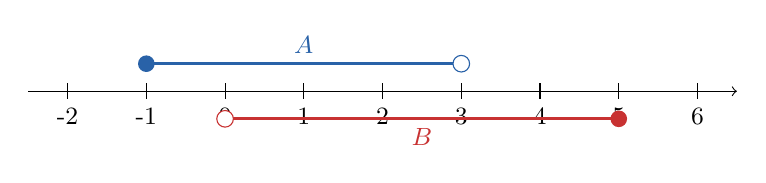
\begin{tikzpicture}
  \draw[->] (-2.5,0) -- (6.5,0);
  \foreach \x in {-2,-1,0,1,2,3,4,5,6}
    \draw (\x, 0.1) -- (\x, -0.1) node[below] {\small \x};

  % A: -1 <= x < 3
  \draw[mainblue, very thick] (-1, 0.35) -- (3, 0.35);
  \fill[mainblue] (-1, 0.35) circle (3pt);
  \draw[mainblue, fill=white] (3, 0.35) circle (3pt);
  \node[mainblue, above] at (1, 0.35) {\small $A$};

  % B: 0 < x <= 5
  \draw[warnred, very thick] (0, -0.35) -- (5, -0.35);
  \draw[warnred, fill=white] (0, -0.35) circle (3pt);
  \fill[warnred] (5, -0.35) circle (3pt);
  \node[warnred, below] at (2.5, -0.35) {\small $B$};
\end{tikzpicture}
\end{center}

$A \cap B$：取 $A$ 和 $B$ 的\textbf{重叠部分}。
\[
A \cap B = \{x \mid 0 < x < 3\}
\]

$A \cup B$：取 $A$ 和 $B$ 的\textbf{合并范围}。
\[
A \cup B = \{x \mid -1 \leqslant x \leqslant 5\}
\]

\begin{tipbox}[数轴法口诀]
\textbf{交集取重叠，并集取覆盖}。画好数轴，注意端点是实心（$\leqslant/\geqslant$，包含）还是空心（$</>$，不包含）。
\end{tipbox}

% 例题6：补集运算
\begin{examplebox}[【例题6】补集运算]
设全集 $U = \{1,\, 2,\, 3,\, 4,\, 5,\, 6,\, 7,\, 8\}$，$A = \{1,\, 3,\, 5,\, 7\}$，求 $\complement_U A$，并验证 $A \cap \complement_U A = \varnothing$，$A \cup \complement_U A = U$。
\end{examplebox}

\textbf{解}：

$\complement_U A$ 是 $U$ 中不属于 $A$ 的元素：
\[
\complement_U A = \{2,\, 4,\, 6,\, 8\}
\]

验证：
\[
A \cap \complement_U A = \{1,3,5,7\} \cap \{2,4,6,8\} = \varnothing \quad\checkmark
\]
\[
A \cup \complement_U A = \{1,2,3,4,5,6,7,8\} = U \quad\checkmark
\]

% 例题7：含参集合问题（简单）
\begin{examplebox}[【例题7】含参集合问题]
设集合 $A = \{x \mid x^2 - 3x + a = 0\}$，若 $A$ 中只有一个元素，求实数 $a$ 的值，并写出集合 $A$。
\end{examplebox}

\textbf{解}：

$A$ 中只有一个元素，说明方程 $x^2 - 3x + a = 0$ 有\textbf{唯一解}（两个相等的实根）。

由判别式 $\Delta = 0$：
\[
\Delta = (-3)^2 - 4 \times 1 \times a = 9 - 4a = 0
\]
\[
a = \frac{9}{4}
\]

此时方程为 $x^2 - 3x + \dfrac{9}{4} = 0$，即 $\left(x - \dfrac{3}{2}\right)^2 = 0$，解为 $x = \dfrac{3}{2}$。

所以 $A = \left\{\dfrac{3}{2}\right\}$。

\begin{warnbox}[易错提醒]
"集合中只有一个元素"不等于"方程只有一个根"。二次方程有唯一解意味着 $\Delta = 0$（两个相等实根），而不是只有一个根、另一个不存在。但如果集合是用一元一次方程定义的，本身就只有一个解，不需要判别式。
\end{warnbox}


% ================================================================
%  第三部分：课堂练习
% ================================================================
\section*{\textcolor{tipgreen}{三、课堂练习}}

\begin{enumerate}[leftmargin=2.5em]
  \item 用列举法表示集合 $C = \{x \mid x^2 - 4 = 0\}$。

  \item 判断下列说法是否正确（对的打 $\checkmark$，错的打 $\times$）：
  \begin{enumerate}[label=(\arabic*)]
    \item $0 \in \varnothing$
    \item $\varnothing \subseteq \{0\}$
    \item $\{1,2\} \subseteq \{1,2,3\}$
    \item $\{1,2,3\} = \{3,2,1\}$
  \end{enumerate}

  \item 设 $A = \{x \mid -2 \leqslant x \leqslant 4\}$，$B = \{x \mid 1 < x < 6\}$，求 $A \cap B$ 和 $A \cup B$。

  \item 设全集 $U = \mathbb{R}$，$A = \{x \mid x \geqslant 2\}$，求 $\complement_U A$。

  \item 写出集合 $\{a,\, b,\, c,\, d\}$ 的所有子集的个数，以及真子集的个数。

  \item 设集合 $P = \{1,\, 2\}$，$Q = \{1,\, 2,\, 3,\, 4\}$，若 $P \subseteq M \subseteq Q$，写出所有满足条件的集合 $M$。
\end{enumerate}

\vspace{10pt}

% ---------- 参考答案 ----------
\begin{knowledgebox}[参考答案]
\textbf{第1题}：

$x^2 - 4 = 0 \implies x = \pm 2$，所以 $C = \{-2,\, 2\}$。

\vspace{6pt}
\textbf{第2题}：
\begin{enumerate}[label=(\arabic*)]
  \item $\times$。空集不含任何元素，所以 $0 \notin \varnothing$。
  \item $\checkmark$。空集是任何集合的子集。
  \item $\checkmark$。$1,2$ 都属于 $\{1,2,3\}$。
  \item $\checkmark$。集合无序，元素相同即相等。
\end{enumerate}

\vspace{6pt}
\textbf{第3题}：

数轴分析：$A = [-2,\, 4]$，$B = (1,\, 6)$。

\[
A \cap B = \{x \mid 1 < x \leqslant 4\}
\]
\[
A \cup B = \{x \mid -2 \leqslant x < 6\}
\]

\vspace{6pt}
\textbf{第4题}：

$\complement_U A = \{x \mid x < 2\} = (-\infty,\, 2)$。

\vspace{6pt}
\textbf{第5题}：

子集个数：$2^4 = 16$ 个；真子集个数：$2^4 - 1 = 15$ 个。

\vspace{6pt}
\textbf{第6题}：

$M$ 必须包含 $1$ 和 $2$，且只能含有 $Q$ 中的元素。因此 $M$ 的可能情况由 $\{3,4\}$ 的子集决定：
\[
M \in \big\{\{1,2\},\;\{1,2,3\},\;\{1,2,4\},\;\{1,2,3,4\}\big\}
\]
共 $4$ 个。
\end{knowledgebox}

\vfill
\begin{center}
\small\textcolor{gray}{本讲义仅供教学参考，例题可根据学生水平调整难度。}
\end{center}

\end{document}
